\documentclass[11pt,preprint, authoryear]{elsarticle}

\usepackage{lmodern}
%%%% My spacing
\usepackage{setspace}
\setstretch{1.2}
\DeclareMathSizes{12}{14}{10}{10}

% Wrap around which gives all figures included the [H] command, or places it "here". This can be tedious to code in Rmarkdown.
\usepackage{float}
\let\origfigure\figure
\let\endorigfigure\endfigure
\renewenvironment{figure}[1][2] {
    \expandafter\origfigure\expandafter[H]
} {
    \endorigfigure
}

\let\origtable\table
\let\endorigtable\endtable
\renewenvironment{table}[1][2] {
    \expandafter\origtable\expandafter[H]
} {
    \endorigtable
}


\usepackage{ifxetex,ifluatex}
\usepackage{fixltx2e} % provides \textsubscript
\ifnum 0\ifxetex 1\fi\ifluatex 1\fi=0 % if pdftex
  \usepackage[T1]{fontenc}
  \usepackage[utf8]{inputenc}
\else % if luatex or xelatex
  \ifxetex
    \usepackage{mathspec}
    \usepackage{xltxtra,xunicode}
  \else
    \usepackage{fontspec}
  \fi
  \defaultfontfeatures{Mapping=tex-text,Scale=MatchLowercase}
  \newcommand{\euro}{€}
\fi

\usepackage{amssymb, amsmath, amsthm, amsfonts}

\def\bibsection{\section*{References}} %%% Make "References" appear before bibliography


\usepackage[round]{natbib}

\usepackage{longtable}
\usepackage[margin=2.3cm,bottom=2cm,top=2.5cm, includefoot]{geometry}
\usepackage{fancyhdr}
\usepackage[bottom, hang, flushmargin]{footmisc}
\usepackage{graphicx}
\numberwithin{equation}{section}
\numberwithin{figure}{section}
\numberwithin{table}{section}
\setlength{\parindent}{0cm}
\setlength{\parskip}{1.3ex plus 0.5ex minus 0.3ex}
\usepackage{textcomp}
\renewcommand{\headrulewidth}{0.2pt}
\renewcommand{\footrulewidth}{0.3pt}

\usepackage{array}
\newcolumntype{x}[1]{>{\centering\arraybackslash\hspace{0pt}}p{#1}}

%%%%  Remove the "preprint submitted to" part. Don't worry about this either, it just looks better without it:
\makeatletter
\def\ps@pprintTitle{%
  \let\@oddhead\@empty
  \let\@evenhead\@empty
  \let\@oddfoot\@empty
  \let\@evenfoot\@oddfoot
}
\makeatother

 \def\tightlist{} % This allows for subbullets!

\usepackage{hyperref}
\hypersetup{breaklinks=true,
            bookmarks=true,
            colorlinks=true,
            citecolor=blue,
            urlcolor=blue,
            linkcolor=blue,
            pdfborder={0 0 0}}


% The following packages allow huxtable to work:
\usepackage{siunitx}
\usepackage{multirow}
\usepackage{hhline}
\usepackage{calc}
\usepackage{tabularx}
\usepackage{booktabs}
\usepackage{caption}


\newenvironment{columns}[1][]{}{}

\newenvironment{column}[1]{\begin{minipage}{#1}\ignorespaces}{%
\end{minipage}
\ifhmode\unskip\fi
\aftergroup\useignorespacesandallpars}

\def\useignorespacesandallpars#1\ignorespaces\fi{%
#1\fi\ignorespacesandallpars}

\makeatletter
\def\ignorespacesandallpars{%
  \@ifnextchar\par
    {\expandafter\ignorespacesandallpars\@gobble}%
    {}%
}
\makeatother

\newlength{\cslhangindent}
\setlength{\cslhangindent}{1.5em}
\newenvironment{CSLReferences}%
  {\setlength{\parindent}{0pt}%
  \everypar{\setlength{\hangindent}{\cslhangindent}}\ignorespaces}%
  {\par}


\urlstyle{same}  % don't use monospace font for urls
\setlength{\parindent}{0pt}
\setlength{\parskip}{6pt plus 2pt minus 1pt}
\setlength{\emergencystretch}{3em}  % prevent overfull lines
\setcounter{secnumdepth}{5}

%%% Use protect on footnotes to avoid problems with footnotes in titles
\let\rmarkdownfootnote\footnote%
\def\footnote{\protect\rmarkdownfootnote}
\IfFileExists{upquote.sty}{\usepackage{upquote}}{}

%%% Include extra packages specified by user

%%% Hard setting column skips for reports - this ensures greater consistency and control over the length settings in the document.
%% page layout
%% paragraphs
\setlength{\baselineskip}{12pt plus 0pt minus 0pt}
\setlength{\parskip}{12pt plus 0pt minus 0pt}
\setlength{\parindent}{0pt plus 0pt minus 0pt}
%% floats
\setlength{\floatsep}{12pt plus 0 pt minus 0pt}
\setlength{\textfloatsep}{20pt plus 0pt minus 0pt}
\setlength{\intextsep}{14pt plus 0pt minus 0pt}
\setlength{\dbltextfloatsep}{20pt plus 0pt minus 0pt}
\setlength{\dblfloatsep}{14pt plus 0pt minus 0pt}
%% maths
\setlength{\abovedisplayskip}{12pt plus 0pt minus 0pt}
\setlength{\belowdisplayskip}{12pt plus 0pt minus 0pt}
%% lists
\setlength{\topsep}{10pt plus 0pt minus 0pt}
\setlength{\partopsep}{3pt plus 0pt minus 0pt}
\setlength{\itemsep}{5pt plus 0pt minus 0pt}
\setlength{\labelsep}{8mm plus 0mm minus 0mm}
\setlength{\parsep}{\the\parskip}
\setlength{\listparindent}{\the\parindent}
%% verbatim
\setlength{\fboxsep}{5pt plus 0pt minus 0pt}



\begin{document}



\begin{frontmatter}  %

\title{Assessing the Effect of the Covid-19 Relief Grant on Household Hunger
using Panel Data Methods - Evidence from NIDS-CRAM}

% Set to FALSE if wanting to remove title (for submission)




\author[Add1]{Johannes Coetsee - 19491050}
\ead{19491050@sun.ac.za}





\address[Add1]{Stellenbosch University}



\vspace{1cm}


\vspace{0.5cm}
\end{frontmatter}



%________________________
% Header and Footers
%%%%%%%%%%%%%%%%%%%%%%%%%%%%%%%%%
\pagestyle{fancy}
\chead{}
\rhead{Econometrics 871 - July 2021}
\lfoot{}
\rfoot{\footnotesize Page \thepage}
\lhead{}
%\rfoot{\footnotesize Page \thepage } % "e.g. Page 2"
\cfoot{}

%\setlength\headheight{30pt}
%%%%%%%%%%%%%%%%%%%%%%%%%%%%%%%%%
%________________________

\headsep 35pt % So that header does not go over title




\hypertarget{introduction}{%
\section{\texorpdfstring{Introduction
\label{Introduction}}{Introduction }}\label{introduction}}

This report attempts to apply and compare panel-data methods to
investigate the effect of the Covid-19 Social Relief of Distress (SRD)
grant on household reported hunger. The SRD is a conditional transfer
implemented to support unemployed individuals who did not receive any
other social grant or UIF (Unemployment Insurance Fund) payment during
the pandemic and ensuing government-instituted lockdowns, and consisted
of 6 monthly payments of R350. Applications for and distribution of the
SRD transfer is managed by South African Social Security Agency (SASSA).
In order to assess the effectiveness of this transfer, it is necessary
to know whether it is successful in providing key social security
outcomes such as food security and self-reported household hunger. The
recent release of the fifth wave of the National Income Dynamics Study -
Coronavirus Rapid Mobile Survey 2020 (NIDS-CRAM) dataset makes it
possible to analyse this effect in a nationally representative context.
Panel-data analysis, afforded by the structure of NIDS-CRAM, could prove
useful in disentangling the effect of the SRD on hunger.

This study compares different static panel model specifications in
estimating this effect: 1) a pooled OLS (POLS) with three varying
specifications, 2) a Fixed Effects (FE) model, 3) First Differences (FD)
model and 4) Random Effects (RE) Model. Throughout, the varying
estimators and specifications will be discussed in terms of their
ability and robustness in obtaining causal effects.\footnote{This study
  attempts to build on similar exploratory analyses such as in Bridgman
  \emph{et al.} (\protect\hyperlink{ref-bridgman2020hunger}{2020}) and
  Köhler \& Hill (\protect\hyperlink{ref-kohler2021distribution}{2021}).}
Results indicate that all methods find the effect of the SRD on
household hunger to be close to 0. These results are robust to replacing
household hunger with other food-insecurity metrics. In terms of model
comparison, however, the FE method is shown to perform the best in
isolating unbiased effects.

\hypertarget{data-and-descriptive-statistics}{%
\section{\texorpdfstring{Data and Descriptive Statistics
\label{Data}}{Data and Descriptive Statistics }}\label{data-and-descriptive-statistics}}

The analysis in this report relies on the National Income Dynamics Study
- Coronavirus Rapid Mobile Survey 2020 (NIDS-CRAM) data, supplied by the
Southern Africa Labour and Development Research Unit (SALDRU) from May
2020 to May 2021. NIDS-CRAM is a nationally representative longitudinal
household survey spanning over five waves, conducted using
Computer-Assisted Telephonic Interviews (CATI), meant to investigate the
impact of the Covid-19 pandemic and subsequent national lockdown on the
South African socioeconomic environment (Ingle \emph{et al.},
\protect\hyperlink{ref-nids2020}{2020}).\footnote{Data is publicly
  available at \url{https://www.datafirst.uct.ac.za/}.} Interviewed
individuals were drawn from the sample members of the fifth wave of
NIDS, following a stratified sampling design. In wave 1, 7073
respondents were interviewed successfully, whilst a top-up of 1084
respondents was added to the sample in wave three due to attrition
between the first and second waves. Lastly, data was collected only on
the individual respondents and no attempt was made at collecting
information from their respective household members, meaning that larger
households are more likely to be interviewed. This sampling structure
therefore only allows for individual-level analysis, although statistics
can be estimated on household living conditions at an individual level,
as is the endeavor of the current study.

As the purpose of this report is to estimate the effect of the SRD on
household-reported hunger, there are two primary variables of
importance, namely, `hunger' - a binary variable where a value of 1
indicates that someone in the interviewed respondent's household (HH)
was hungry in the last 7 days - and `c19grant' - a binary variable where
a value of 1 indicates whether the respondent lives in a household that
receives at least one SRD grant. Figure \ref{hunger} below outlines the
proportion of the South African population that have experienced food
insecurity and hunger over the five waves of NIDS-CRAM. There seems to
be downward trends in the proportion of individuals that report hunger
in at least one person in their household, as well as in child hunger.
It is also interesting to note that child-hunger is much lower than the
reported household hunger. Lastly, and although trending downward over
time, respondents report there to be no money for food in nearly 30\% of
households in almost all of the waves. When viewed together, the
statistics on these metrics indicate that food security should be a
concern for policy-makers during the Covid-19 era. That is, in essence,
one of the justifications of an expansion of the social security
framework to include the SRD transfer. Figure \ref{grant} below shows
the take-up of this grant over time.\footnote{The grant was not yet paid
  out during the first wave, which explains its absence here.} It is
notable that the proportion of individuals who received the transfer, or
lives with someone who receives it, has increased from 0 in wave 1 to
almost 24\% in wave 5.

\begin{figure}[H]
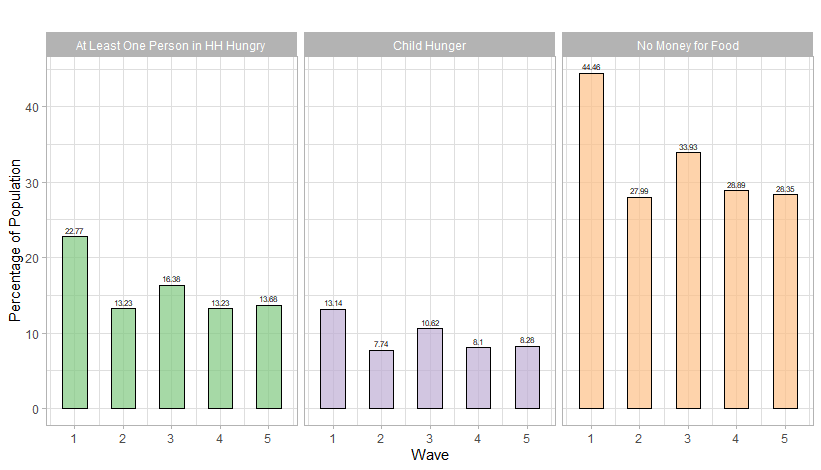
\includegraphics[width=1\linewidth]{figures/hunger_descrip} \caption{\label{hunger} Descriptive Statistics on Hunger}\label{fig:hunger}
\end{figure}

\begin{figure}[H]
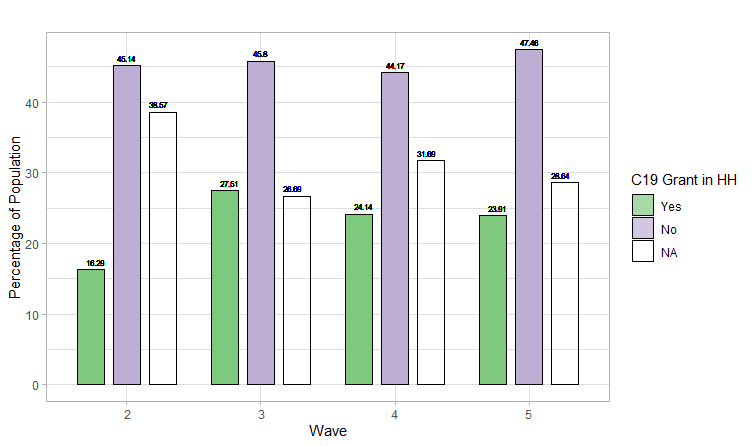
\includegraphics[width=1\linewidth]{figures/c19_grant_descrip} \caption{\label{grant} Proportion of SRD Recipients}\label{fig:grant}
\end{figure}

\hypertarget{methodology}{%
\section{\texorpdfstring{Methodology
\label{Meth}}{Methodology }}\label{methodology}}

As mentioned in Section \ref{Introduction}, this paper compares four
static panel models with regards to their robustness in estimating the
effect of the SRD on household hunger. In order to account for the
complex survey design and related attrition and non-random response
discussed in the previous section, panel weights are employed for panel
methods, while the original NIDS cluster and strata variables were used
throughout.\footnote{This is according to the guidelines for
  longitudinal analysis set out in Ingle \emph{et al.}
  (\protect\hyperlink{ref-nids2020}{2020}), where panel weights excludes
  wave three top-up members, and is scaled to the NIDS wave 5
  population. For the POLS specifications, weights include the top-up
  members.} The pooled OLS models - of which there are three differing
specifications - attempt to control on observables by using variation
between individuals to isolate causal effects, whilst assuming that
unobservables are independently distributed, and constitutes the
baseline specifications that the panel models are compared
against.\footnote{The more technical aspects of this section is
  elucidated further in Wooldridge
  (\protect\hyperlink{ref-wooldridge}{2015}).}

After merging the data across waves and setting the survey design
according to that specified above, the models are estimated. The first,
a baseline pooled OLS, regresses hunger on the primary independent
variable, c19grant. However, this specification is problematic. For
instance, omitted variable bias is introduced when treatment is
correlated with other covariates that are not controlled for, such as,
for instance, whether the household receives other grants, the size of
the household, or the average HH income. Failure to control for these
variables would violate the identifying assumption of OLS, as the effect
of the SRD grant might be masked by these other covariates. The second
POLS specification thereby include these controls - HH size, HH income
and whether HHs receive grants.\footnote{It must be remembered that the
  SRD transfer is only granted to those who do not receive other
  transfers from government or employment income. However, the c19grant
  variable used in this analysis incorporates whether other household
  members receive such a grant, thereby necessitating the inclusion of
  other covariates that would have been nullified - such as household
  income - due to the conditional nature of the transfer.} The third
POLS model includes time dummies to control for the time trend, and
other covariates such as the province of residence and the respondent's
race, gender, age, highest attained education level, and whether the
dwelling is in a rural or urban setting, as these factors may all
introduce bias through their possible correlation with SRD.\footnote{For
  instance, persons who have attained higher education would be more
  likely to find the SRD application process easier to manage, as well
  as being less likely to be hungry (due to possibly being more
  resourceful in finding food).} All standard errors for the OLS models
are clustered at the individual level due to repeated observations of
the same individual across waves.

Whilst the specifications above control for some observable
characteristics, it cannot control for possible selection on
unobservables. For instance, it is feasible to imagine that those
individuals who are more likely to become hungry due to anatomical
differences, or those more likely to vocalize their hunger compared to
others, are also more likely to apply for the SRD. The fact that
households can move in and out of receiving a SRD grant across waves
makes it possible to estimate the effect of the grant on hunger using FE
estimation. However, time-persistent variables will offer no information
from which to inform estimation, meaning that only the within-level
variation remains. The assumptions underlying FE estimation - weak
unconfoundedness, where the the error term must be uncorrelated with the
observable predictors, and the same trends assumption, where the time
trend may not depend on treatment status - both hold intuitively in this
case. It is unlikely that time-variant unobservables can induce omitted
variable bias. The third model employs a first-differencing methodology,
an alternative to the demeaning process used by FE estimation. However,
FD requires strict exogeneity of the regressors, and is also prone to
inconsistent estimation if explanatory variables are subject to
measurement error. In the NIDS-CRAM dataset, the possibility of
measurement error is likely fairly high due to the telephonic
interviewing procedure. Lastly, a RE model is estimated. REs are more
efficient than any other specification above, given that it reports
smaller standard errors. However, RE only delivers unbiased results in
the case of strict exogeneity, otherwise delivering inconsistent
estimates. In order to assess whether this is the case, Hausman tests
are performed to compare FE and RE models.

Finally, as an additional robustness check, models are also estimated
for two other metrics of food insecurity, namely, `household child
hunger' and `having no money for food'. After estimation, models will be
compared as to the economic and statistical significance of their
coefficients, as well as the likelihood of core assumptions being
violated. The results of all specifications are displayed in the
following section.

\hypertarget{results}{%
\section{\texorpdfstring{Results
\label{Results}}{Results }}\label{results}}

Table \ref{results} below presents the results of the three POLS models
and three other static panel models considered. Results as a whole seem
to indicate a negligible causal effect attributable to having at least
one person in the HH that have received the SRD grant on whether anyone
in the household was reported as hungry. The coefficients from the POLS
models display a positive effect of the grant on household hunger where
one would expect it to be negative, perhaps indicating that the POLS
specifications are biased upwards due to unobservables. The effect of
household income and household size is also surprisingly small, given
that one would expect household income to be correlated with both SRD
grants and hunger. Furthermore, the c19grant coefficient decreases when
adding more controls to the first POLS model, albeit whilst also losing
statistical insignificant. It is also important to note that the
wave-dummy coefficients are insignificant, and also 0 in some cases.
This might be due to collinearity, making the third model less
attractive in isolating a causal effect.

The FE specification - Model 4 - also produces a small coefficient value
for the SRD grant, but is of the expected negative sign and is
statistically significant at the 10\% level. The FD model displays a
lower coefficient than the previous models, whilst also not being
statistically significant. Moreover, the sample size for the FD is lower
than for the other models due to the unbalanced nature of the data,
which, although not problematic, means that the FD model has less
information to draw inference from. Lastly, the RE model coefficient is
the closest to 0 out of all models, and is statistically insignificant.
When comparing the FE and RE coefficients, it is important to note that
they differ relatively in size, indicating that exogeneity might not
hold for both models. A Hausman test, displayed in the appendix (Table
\ref{hausman}), shows that one can reject the null hypothesis of
exogeneity being present at a 1\% level, further justifying FE to be
more appropriate than RE in this context.

\begin{figure}[H]
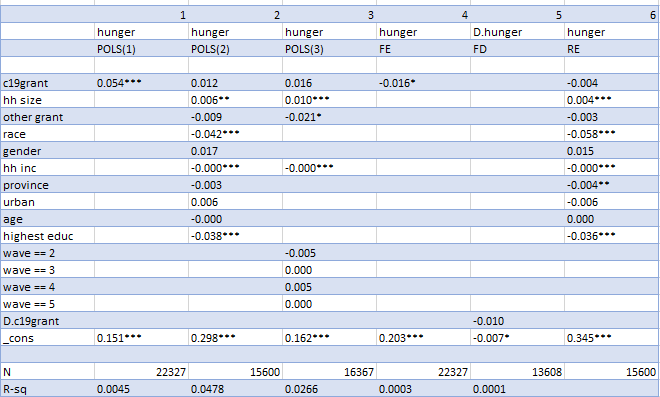
\includegraphics[width=1\linewidth]{figures/hunger_table} \caption{\label{results} Estimation Results (Own Calculations, Data: NIDS-CRAM)}\label{fig:results}
\end{figure}

It is clear that the effect of SRD on hunger is negligibly close to 0
across all specifications. These results are substantiated further when
substituting out different measures for food insecurity, the results of
which are displayed in the appendix \ref{appendix}. Using all three
different measures, and across all models, the effect remains close to
zero.\footnote{Hausman tests for these other metrics also indicate FE to
  be more appropriate.} Bridgman \emph{et al.}
(\protect\hyperlink{ref-bridgman2020hunger}{2020}) reports similar
results, concluding that the small effect might be due to the monetary
value of R350 not being sufficient to lift households above food
security lines. It is also possible that individuals that receive the
grant do not distribute the gains to other members of the household,
thereby not reducing reported hunger in other household members.

In terms of model comparison, however, it seems as if the FE model is
the most robust in approaching an unbiased effect of the SRD grant on
household hunger, regardless of the food security metric. This is due to
the FE identifying assumptions being the least likely to be violated,
given that FE does not require strict exogeneity like the RE or FD
models, whilst also accounting for selection on unobservables, which
POLS cannot offer. Similarly, FE displays significant results and
similar coefficient values across the differing metrics.

\hypertarget{discussion}{%
\section{\texorpdfstring{Discussion
\label{Discussion}}{Discussion }}\label{discussion}}

This report compared the success of four different specifications in
isolating the causal effect of the Special Relief of Distress (SRD)
grant on household hunger using the longitudinal NIDS-CRAM dataset.
Initial exploratory results indicate a negligible effect across all
specifications, and across various food-insecurity and hunger measures.
It is also shown that the FE estimation method seems to be the most
robust in estimating an unbiased causal effect, as it controls for
selection on unobservables, whilst its primary assumptions of common
trend over time and weak unconfoundedness are less likely to be
violated. There remains much scope for further analysis and checks for
robustness. For instance, one could compare these results to those
obtained for a similar study where the household receipt of SRD is
replaced by personal receipt of the SRD. If the results from the latter
estimation are economically more significant than for the prior
estimation, it might give an indication on the makeup of resource
distribution within households.

\newpage

\hypertarget{references}{%
\section*{References}\label{references}}
\addcontentsline{toc}{section}{References}

\hypertarget{refs}{}
\leavevmode\hypertarget{ref-bridgman2020hunger}{}%
Bridgman, G., Van der Berg, S., Patel, L. \& others. 2020. \emph{Hunger
in south africa during 2020: Results from wave 2 of nids-cram}. ed.
Department of Economics, University of Stellenbosch.

\leavevmode\hypertarget{ref-nids2020}{}%
Ingle, K., Brophy, T. \& Daniels, R. 2020. National income dynamics
study--coronavirus rapid mobile survey (nids-cram) panel user manual.
\emph{Technical Note Version}. 1.

\leavevmode\hypertarget{ref-kohler2021distribution}{}%
Köhler, T. \& Hill, R. 2021. The distribution and dynamics of south
africa's ters policy.

\leavevmode\hypertarget{ref-wooldridge}{}%
Wooldridge, J.M. 2015. \emph{Introductory econometrics: A modern
approach}. ed. Cengage learning.

\newpage

\hypertarget{appendix}{%
\section*{\texorpdfstring{Appendix
\label{appendix}}{Appendix }}\label{appendix}}
\addcontentsline{toc}{section}{Appendix \label{appendix}}

\begin{figure}[H]
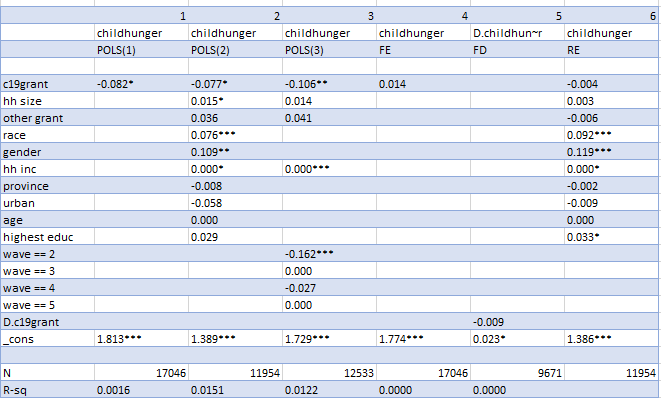
\includegraphics[width=1\linewidth]{figures/childhunger_table} \caption{\label{results_child} Table of Results - Child Hunger (Own Calculations, Data: NIDS-CRAM)}\label{fig:results_child}
\end{figure}

\begin{figure}[H]
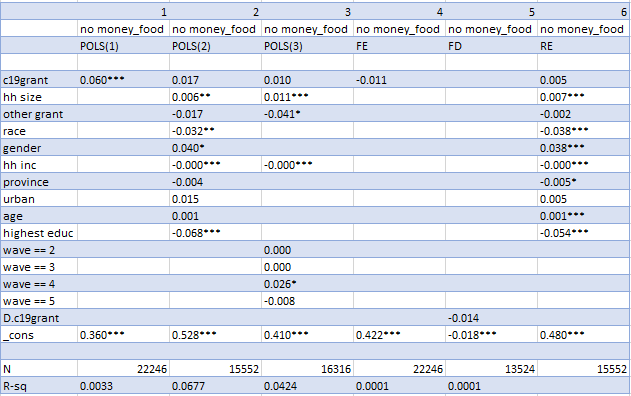
\includegraphics[width=1\linewidth]{figures/nomoney_table} \caption{\label{results_money} Table of Results - No Money For Food (Own Calculations, Data: NIDS-CRAM)}\label{fig:results_money}
\end{figure}

\begin{figure}[H]
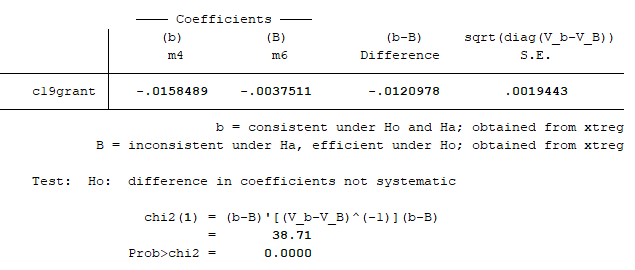
\includegraphics[width=1\linewidth]{figures/hausman1} \caption{\label{hausman} Hausman Test (Own Calculations, Data: NIDS-CRAM)}\label{fig:hausman}
\end{figure}

\bibliography{Tex/ref}





\end{document}
